%\documentclass[handout]{beamer}\mode<handout>{\usetheme{default}}
%
\documentclass[presentation]{beamer}\mode<presentation>{\usetheme{AMSBolognaFC}}
%\documentclass[handout]{beamer}\mode<handout>{\usetheme{AMSBolognaFC}}
%%%%%%%%%%%%%%%%%%%%%%%%%%%%%%%%%%%%%%%%%%%%%%%%%%%%%%%%%%%%%%%%%%%%%%%%%%%%%%%%
%\setbeamertemplate{bibliography item}{\insertbiblabel}
\usepackage{plp-aixia-2021-talk}
%%%%%%%%%%%%%%%%%%%%%%%%%%%%%%%%%%%%%%%%%%%%%%%%%%%%%%%%%%%%%%%%%%%%%%%%%%%%%%%%
\title[PLP in \twopkt{}]{Probabilistic Logic Programming in \twopkt{}}
%
\author[Dellaluce \and Calegari \and \sspeaker{Ciatto}]{
    Jason Dellaluce$^*$ \and Roberta Calegari$^\dagger$ \and \speaker{Giovanni Ciatto}$^*$
    \\\smallskip\small
    \email{jason.dellaluce@studio.unibo.it} \and \email{roberta.calegari@unibo.it} \and \speaker{\email{giovanni.ciatto@unibo.it}}
}
%
\institute[UniBO]{
    $^*$ \disi
    \\
    $^\dagger$ \almaai
    \\
    $^{*\dagger}$ \unibo
}
%
\date[AIxIA, Dec. 1, 2021]{
    $20^{th}$ International Conference of the
    \\
    Italian Association for Artificial Intelligence (AIxIA)
    \\\medskip
    Milan, 2021-12-01 (Virtual Conference)
}
%
%%%%%%%%%%%%%%%%%%%%%%%%%%%%%%%%%%%%%%%%%%%%%%%%%%%%%%%%%%%%%%%%%%%%%%%%%%%%%%%%
\begin{document}
%%%%%%%%%%%%%%%%%%%%%%%%%%%%%%%%%%%%%%%%%%%%%%%%%%%%%%%%%%%%%%%%%%%%%%%%%%%%%%%%

%/////////
\frame{\titlepage}
%/////////

%===============================================================================
\section*{Outline}
%===============================================================================

%/////////
\frame[c]{\tableofcontents[hideallsubsections]}
%/////////

%===============================================================================
\section{Motivation, Context, and Goals}
%===============================================================================

\subsection{Context}

%/////////
\begin{frame}[c]{Context}
    \begin{block}{\textbf{Probabilistic logic programming} (PLP)\ccite{riguzzi2018}}
        \begin{itemize}
            \item programming \alert{paradigm} rooted in computational logic
            \item \alert{probabilistic} theories as programs
            \item logic \alert{inference} used to
            %
            \begin{enumerate}
                \item \alert{compute probabilities} for logic \alert{queries}
                \item \alert{tune} probabilistic models from \alert{data}
            \end{enumerate}
        \end{itemize}
    \end{block}
    %
    \begin{block}{In this paper}
        \begin{itemize}
            \item we focus on the \alert{resolution} of probabilistic queries
            \item from a \alert{technological} perspective
        \end{itemize}
    \end{block}
\end{frame}
%/////////

\subsection{Motivation}

%/////////
\begin{frame}[c]{Motivations}

    \begin{enumerate}
        \item Current technologies for (P)LP are \alert{technological \emph{silos}}
        %
        \begin{itemize}
            \item poor \alert{inter-platform} interoperability
            \item (P)LP facilities cannot simply be exploited \alert{``as a library''}
        \end{itemize}

        \bigskip

        \item Hard to exploit (P)LP in \alert{mainstream} programming

        \bigskip

        \item Willing to extend the \alert{\twopkt{}} ecosystem\ccite{2pkt-swx16} towards PLP
        %
        \begin{itemize}
            \item our \alert{inherently multi-platform} LP ecosystem
        \end{itemize}

        \bigskip

        \item \alert{Call to arms} for anyone interested in joining our efforts

    \end{enumerate}

\end{frame}
%/////////

\subsection{Background}

%/////////
\begin{frame}[c]{Background -- PLP}

    \begin{itemize}
        \item Two major technologies for PLP: $\begin{cases}
            \text{\problog\ccite{de-raedt-2007}}
            \\
            \text{\cplint\ccite{riguzzi-2007}}
        \end{cases}$

        \bigskip

        \item Both based on
        %
        \begin{itemize}
            \item logic programs with annotated disjunctions\ccite{de-raedt-2007} (\alert{LPAD})

            \item Sato's \alert{distribution semantics}\ccite{sato1995}
        \end{itemize}

        \bigskip

        \item Both relying on \alert{knowledge compilation}\ccite{darwiche2002knowledge} to reach efficiency
        %
        \begin{itemize}
            \item namely, onto (some variant of) binary decision diagrams\ccite{akers1978binary} (\alert{BDD})
        \end{itemize}

        \bigskip

        \item Both exploiting some \alert{Prolog technology} behind the scenes
        %
        \begin{itemize}
            \item \problog{} $\longrightarrow$ YAP Prolog\ccite{CostaRD12}
            \item \cplint{} $\longrightarrow$ SWI-Prolog\ccite{WielemakerSTL12}
        \end{itemize}

    \end{itemize}

\end{frame}
%/////////

%/////////
\begin{frame}[c]{Background -- \twopkt{}\ccite{2pkt-swx16} \hfill \uurl{https://github.com/tuProlog/2p-kt}}

    \begin{center}
        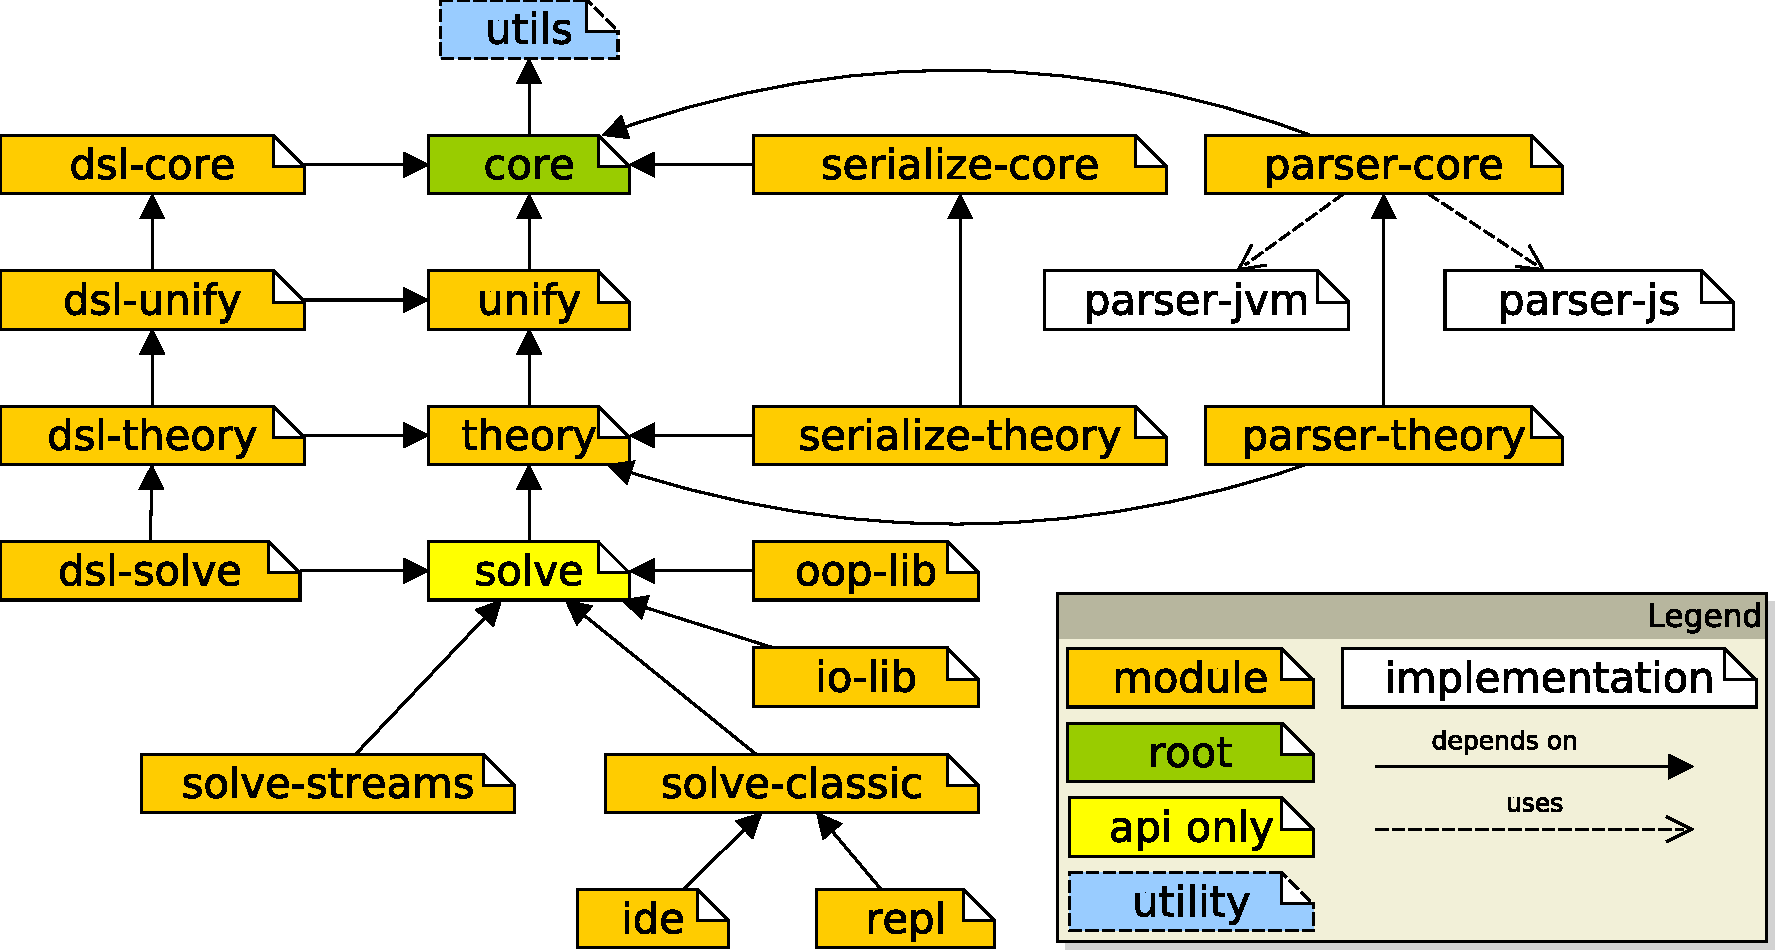
\includegraphics[width=.7\linewidth]{img/project-map.pdf}
    \end{center}
    %
    \begin{itemize}\small
        \item Collection of general-purpose modules for LP
        \item Supporting LP facilities individually, \alert{as a library}
        \item Multi-platform support: JVM, JavaScript, Android, Python\footnotemark
    \end{itemize}

    \footnotetext{\url{https://github.com/tuProlog/2ppy}}

\end{frame}
%/////////

\subsection{Contribution}

%/////////
\begin{frame}[c]{Contribution of this work}

    \begin{enumerate}
        \item Extend \twopkt{} towards PLP support
        %
        \begin{itemize}
            \item design an agnostic API for PLP
            \item custom implementation of \problog{}
        \end{itemize}

        \vfill

        \item Make PLP exploitable as a library\ldots

        \vfill

        \item \ldots on as many platforms as possible
        %
        \begin{itemize}
            \item namely, JVM, JavaScript, Android, and Python
        \end{itemize}

    \end{enumerate}

\end{frame}
%/////////

%===============================================================================
\section{Contribution: PLP on \twopkt{}}
%===============================================================================

%/////////
\begin{frame}[c]{Overview -- What we added}


    \begin{center}
        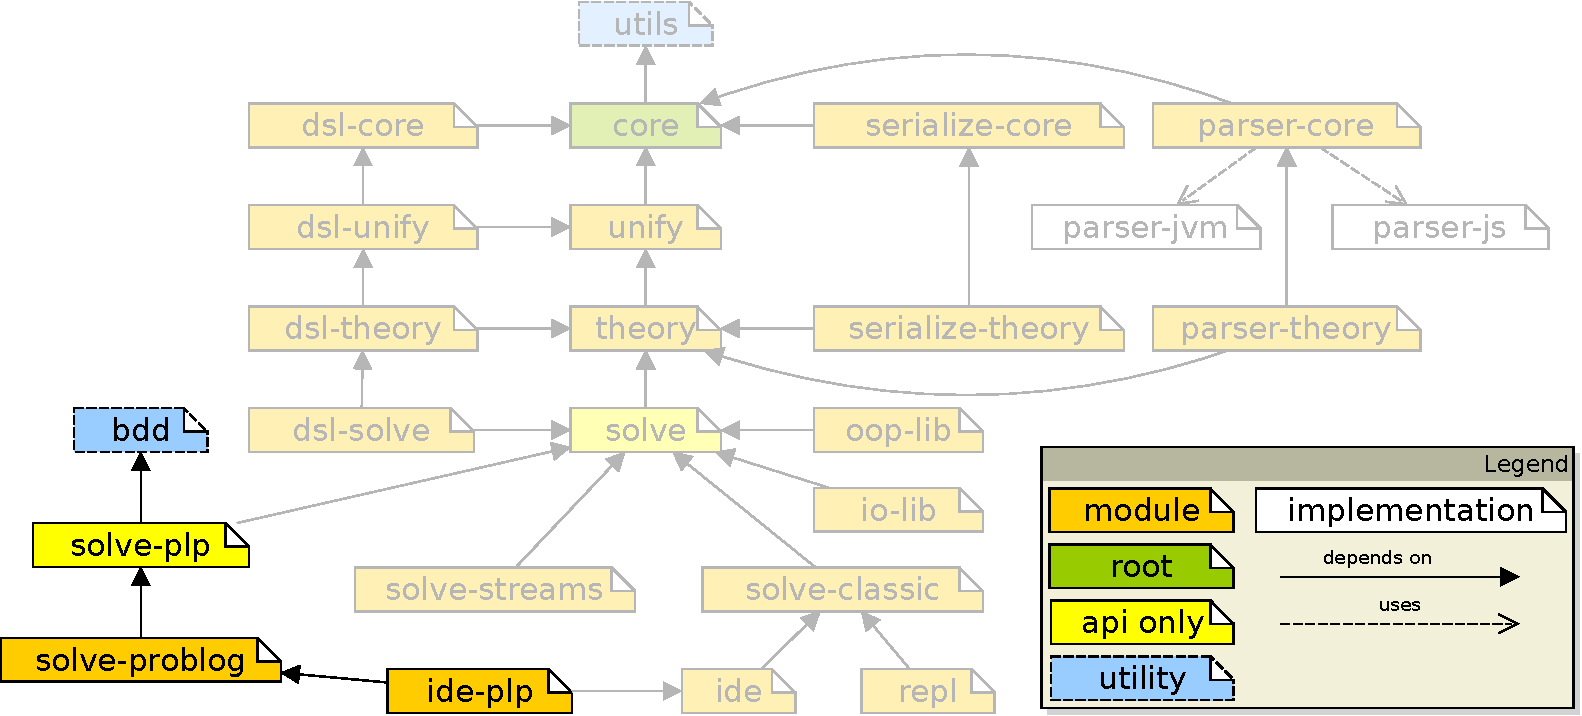
\includegraphics[width=.7\linewidth]{img/project-map-diff.pdf}
    \end{center}
    %
    \begin{description}\small
        \item[\module{bdd}] multi-platform implementation of BDD
        %
        \item[\module{solve-plp}] general API for PLP
        %
        \item[\module{solve-problog}] multi-platform implementation of \problog{}
        %
        \item[\module{ide-plp}] graphical user interface for PLP
    \end{description}

\end{frame}
%/////////

\subsection{Design}


%/////////
\begin{frame}[c]{Our custom \problog{} solver}

    \begin{columns}
        \begin{column}{.5\linewidth}
            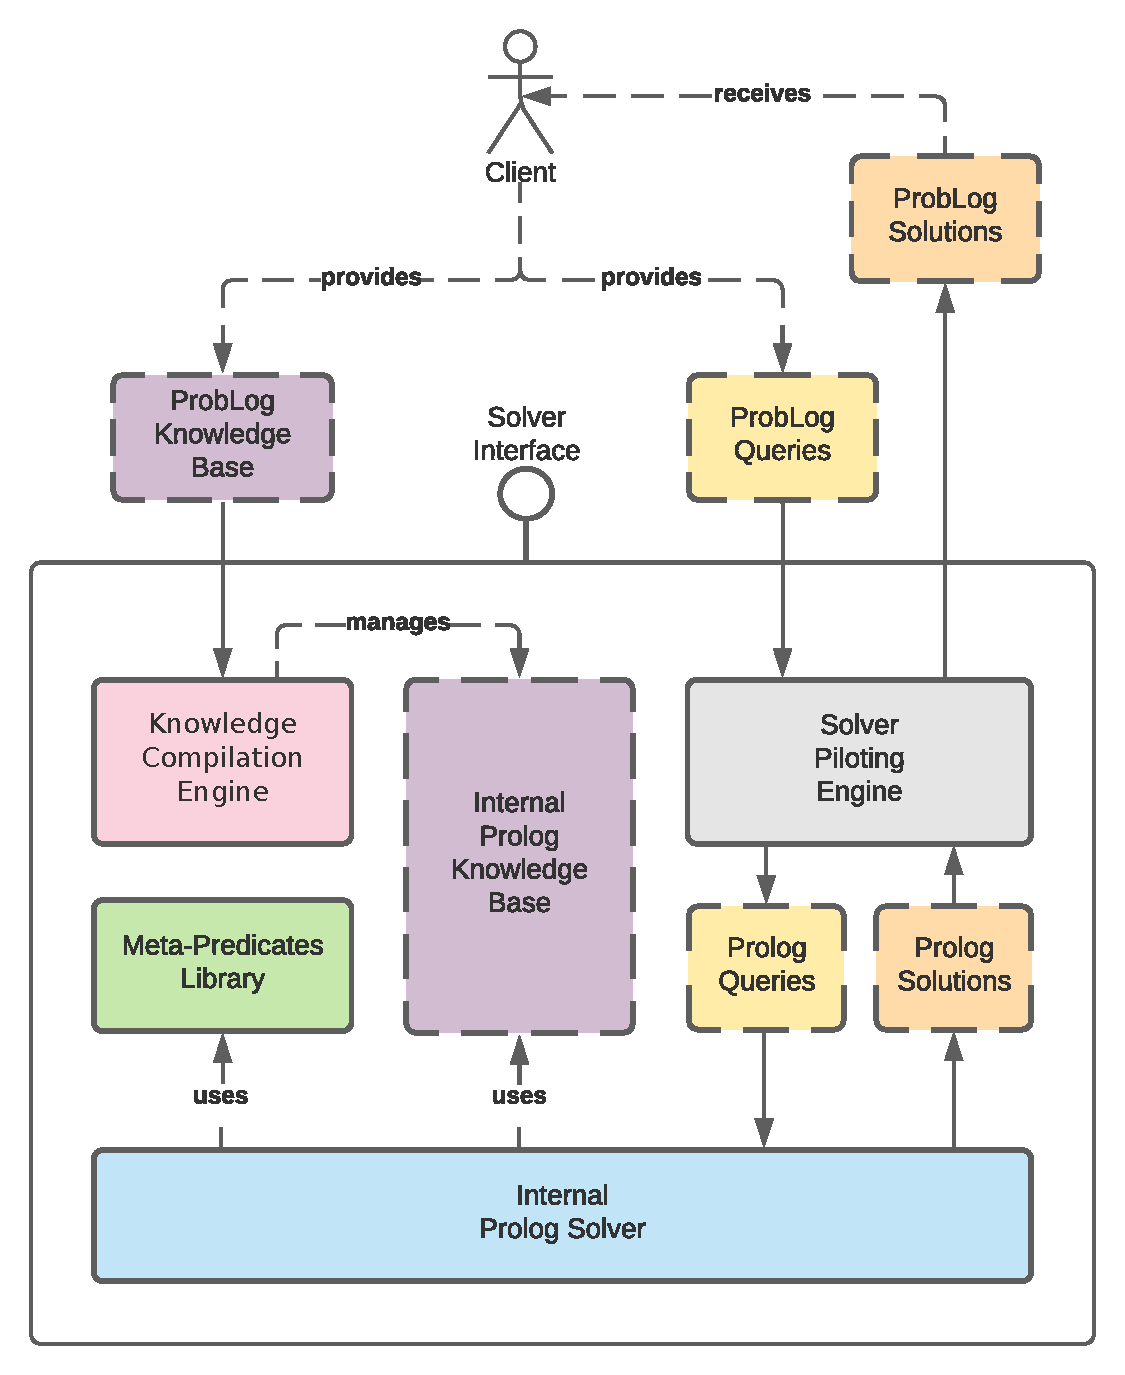
\includegraphics[width=\linewidth]{img/design-problog-architecture.pdf}
        \end{column}
        \hfill
        \begin{column}{.5\linewidth}
            Major components:
            %
            \medskip
            %
            \begin{enumerate}
                \item knowledge compilation engine
                \medskip
                \item library of meta-predicates
                \medskip
                \item solver piloting engine
            \end{enumerate}
        \end{column}
    \end{columns}

\end{frame}
%/////////

%/////////
\begin{frame}[c, allowframebreaks]{Knowledge Compilation Engine}

    \begin{block}{Re-writing rules}
        \begin{adjustbox}{width=\textwidth,center}
            \begin{tabular}{rcl}
                \encode{\pl{$f(\bar{X})$.}} & $\longrightarrow$ & `\pl{prob(\textit{E}, $f(\bar{X})$) :- expl\_build(\textit{E}, 1.0).}'
                \\
                \encode{\pl{$p$::$f(\bar{X})$.}} & $\longrightarrow$ & `\pl{prob(\textit{E}, $f(\bar{X})$) :- expl\_build(\textit{E}, $p$).}'
                \\
                \encode{\pl{$p$::$f(\bar{X})$ :- $b_1(\bar{X}_1)$, \ldots, $b_n(\bar{X}_n)$.}} & $\longrightarrow$ & `\pl{prob(\textit{E}, $f(\bar{X})$) :-} \pl{expl\_build(\textit{E}$_0$, $p$),} \\
                & & \qquad \pl{prob(\textit{E}$_1$, $b_1(\bar{X}_1)$),} \ldots\pl{, prob(\textit{E}$_n$, $b_n(\bar{X}_n)$),} \\
                & & \qquad \pl{expl\_and(\textit{E}, [\textit{E}$_0$, \textit{E}$_1$, \ldots, \textit{E}$_n$]).}'
                \\
                \encode{\pl{$p_1$::$f_1(\bar{X}_1)$, \ldots, $p_m$::$f_m(\bar{X}_m)$ :- $\bar{b}$.}} & $\longrightarrow$ & `\encode{\pl{$p_1$::$f_1(\bar{X}_1)$ :- $\bar{b}$.}}\pl{.} \ldots \encode{\pl{$p_m$::$f_m(\bar{X}_m)$ :- $\bar{b}$.}}\pl{.}' \\
            \end{tabular}
        \end{adjustbox}
    \end{block}

    \begin{figure}
        \fbox{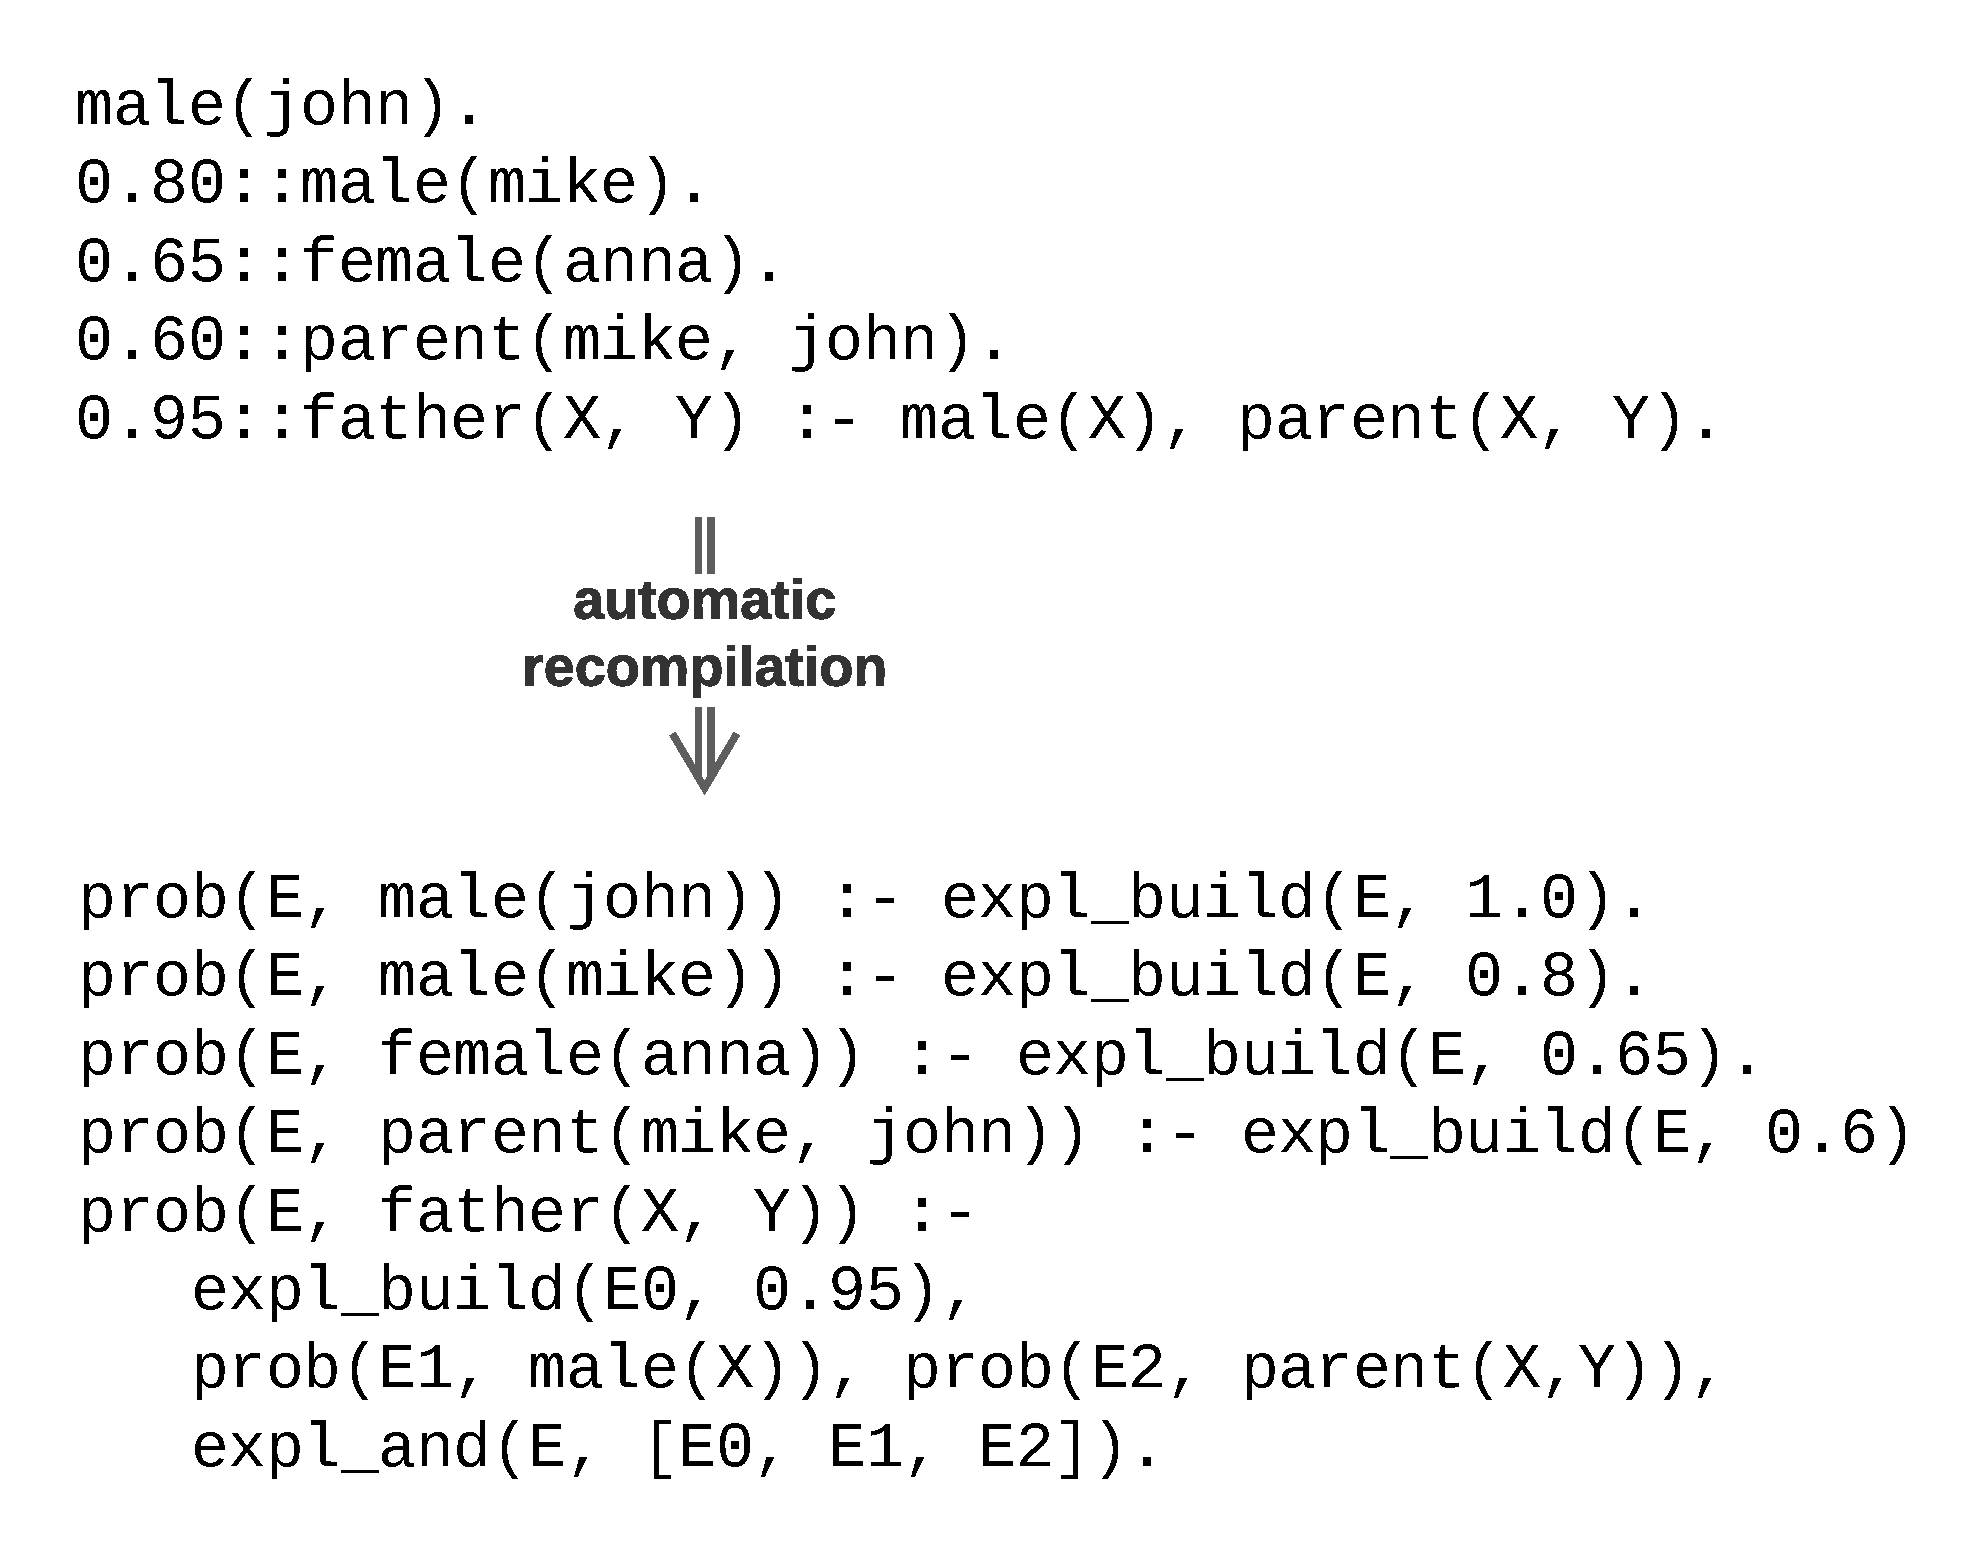
\includegraphics[width=.5\linewidth]{img/design-problog-theory-transformation.pdf}}
        \caption{Example of knowledge compilation}
    \end{figure}

\end{frame}
%/////////

%/////////
\begin{frame}[c]{Library of meta-predicates}

    \begin{description}
        \item[\pl{expl\_and(-\textit{E}, [+\textit{E}$_1$, \ldots, +\textit{E}$_n$])}] for conjunction

        \vfill

        \item[\pl{expl\_or(-\textit{E}, [+\textit{E}$_1$, \ldots, +\textit{E}$_n$])}] for disjunction

        \vfill

        \item[\pl{expl\_not(-\textit{E}, +\textit{E}$'$)}] for negation

        \vfill

        \item[\pl{expl\_build(-\textit{E}, +\textit{P})}] for facts' probabilities

        \vfill

        \item[\pl{prolog\_query(-\textit{Probability}, +\textit{Goal})}] for perform probabilistic queries
    \end{description}

    \vfill

    \begin{alertblock}{Assumptions}
        \begin{itemize}
            \item explanations consist of BDD, represented as constant terms in logic
            \item BDD are manipulated in Kotlin, via \alert{generators}\ccite{2pkt-jelia2021}
        \end{itemize}
    \end{alertblock}

\end{frame}
%/////////

%/////////
\begin{frame}[c]{Solver Piloting Engine}


    \begin{center}
        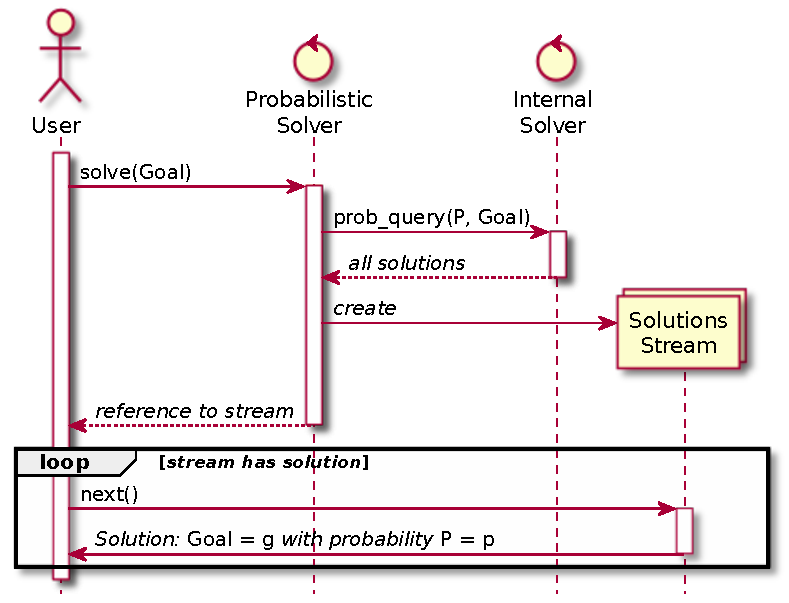
\includegraphics[width=.5\linewidth]{img/general-api.pdf}
    \end{center}
    %
    \begin{itemize}\small
        \item Probabilistic solvers are queried with a \alert{goal}
        \item They respond with \alert{variables assignments} and their \alert{probabilities}
        \item An \alert{internal solver} may be exploited behind the scenes to compute solutions
    \end{itemize}

\end{frame}
%/////////

%===============================================================================
\section{Results}
%===============================================================================

%/////////
\begin{frame}[c, allowframebreaks]{Results}

    \begin{block}{In a nutshell}
        \begin{itemize}
            \item Our PLP implementation can be used \alert{as a language}\footnotemark\ldots

            \footnotetext{\tiny cf. \url{https://github.com/tuProlog/2p-kt/releases/latest}}

            \item \ldots or as a library\footnotemark on Java, Kotlin, JavaScript, and Python

            \footnotetext{\tiny cf. \url{https://github.com/tuProlog/2pkt-problog-compatibility-demo}}
        \end{itemize}
    \end{block}

    \begin{figure}
        \centering
        \begin{subfigure}{0.4\linewidth}
            \caption{}
            \label{fig:problog-ide:screenshot}
            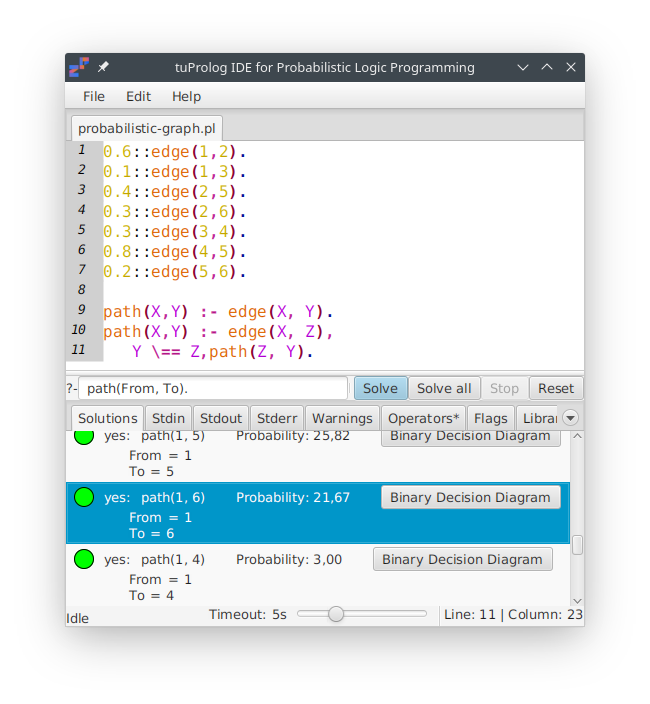
\includegraphics[width=\linewidth]{img/valid-ide-screenshot.png}
        \end{subfigure}
        %
        \hfill
        %
        \begin{subfigure}{0.59\linewidth}
            \caption{}
            \label{fig:problog-ide:graph}
            \fbox{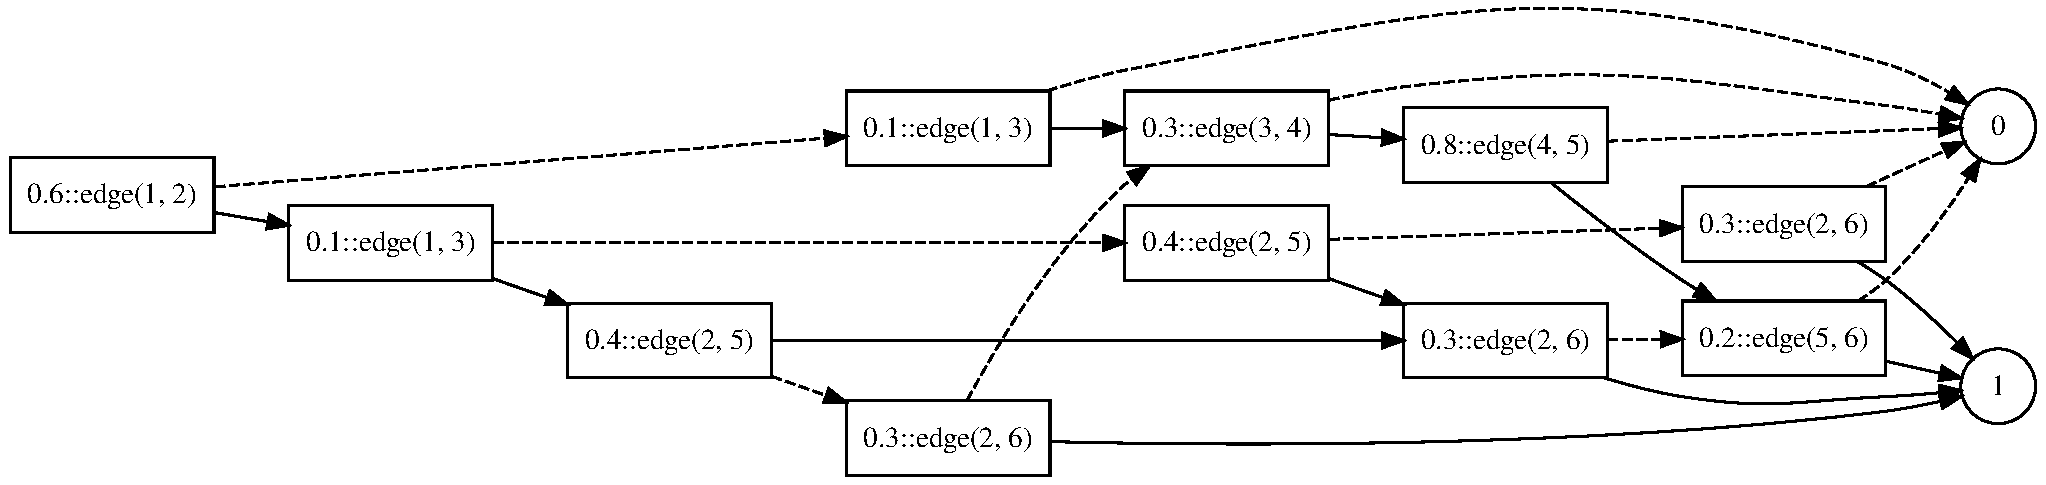
\includegraphics[width=\linewidth]{img/valid-bdd-h.pdf}}
        \end{subfigure}
        \caption{\twopkt{} PLP IDE (\ref{fig:problog-ide:screenshot}) and corresponding BDD built by the solver (\ref{fig:problog-ide:graph})}
        \label{fig:problog-ide}
    \end{figure}

    Usage as a library:

    \lstinputlisting[language=Kotlin, basicstyle=\tiny\ttfamily, label={lst:probabilistic-graph-kt}]{listings/probabilistic-graph.kt}

    \lstinputlisting[language=Java, basicstyle=\tiny\ttfamily, label={lst:probabilistic-graph-kt}]{listings/probabilistic-graph.java}

    \lstinputlisting[language=Python, basicstyle=\tiny\ttfamily, label={lst:probabilistic-graph-py}]{listings/probabilistic-graph.py}

    \lstinputlisting[language=JavaScript, basicstyle=\tiny\ttfamily, label={lst:probabilistic-graph-js}]{listings/probabilistic-graph.js}

\end{frame}
%/////////

%===============================================================================
\section{Conclusions and Future Works}
%===============================================================================

%/////////
\begin{frame}[c]{Conclusions and Future Works}

    \begin{block}{Summing up, in this paper we}
        \begin{itemize}
            \item design and implemented a \alert{\problog{} module} for \twopkt{}
            \item bringing \alert{PLP as a library} to \alert{many platforms}/languages
        \end{itemize}
    \end{block}

    \begin{exampleblock}{In the future we plan to}
        \begin{itemize}
            \item gain efficiency by removing the \alert{knowledge re-compilation} step
            \item support \alert{approximate} resolution
            \item explore the exploitation of \alert{MDD} instead of BDD
        \end{itemize}
    \end{exampleblock}

\end{frame}
%/////////


%===============================================================================
\section*{}
%===============================================================================

%/////////
\frame{\titlepage}
%/////////

%===============================================================================
\section*{\refname}
%===============================================================================

%%%%
\setbeamertemplate{page number in head/foot}{}
%/////////
%\begin{frame}[c,noframenumbering]{\refname}
\begin{frame}[t,allowframebreaks,noframenumbering]{\refname}
%	\tiny
	\scriptsize
%	\footnotesize
%	\bibliographystyle{plain}
	\bibliographystyle{alpha}
	\bibliography{plp-aixia-2021-talk}
\end{frame}
%/////////

%%%%%%%%%%%%%%%%%%%%%%%%%%%%%%%%%%%%%%%%%%%%%%%%%%%%%%%%%%%%%%%%%%%%%%%%%%%%%%%%
\end{document}
%%%%%%%%%%%%%%%%%%%%%%%%%%%%%%%%%%%%%%%%%%%%%%%%%%%%%%%%%%%%%%%%%%%%%%%%%%%%%%%%
